\def \kaflanr {22}
\lecture[\kaflanr]{\kaflanr. Heildi vigursviðs yfir flöt}{lecture-text}
\date{18.~mars 2015}
\newcounter{mycount}
\refstepcounter{mycount}

\begin{document}

\begin{frame}
	\maketitle
\end{frame}




\begin{frame}{Einingarþvervigrasvið} 

\begin {block}{Skilgreining \rtask{}}

Látum $\cal S$ vera flöt í $\R^3$.  {\em Einingarþvervigur} $\nv$ á flötinn
$\cal S$ í punktinum $P$ er einingarvigur hornréttur á
snertiplan við flötinn í punktinum $P$.  

{\em Einingarþvervigrasvið} á
$\cal S$ er samfellt vigursvið $\Nv$ sem er skilgreint í öllum punktum
$\cal S$ þannig að fyrir $(x,y,z)\in{\cal S}$ er vigurinn $\nv(x,y,z)$
einingarvigur sem er hornréttur á snertiplan við flötinn í punktinum
$(x,y,z)$.
\end{block}
\begin {figure}[h!]
 \centering
            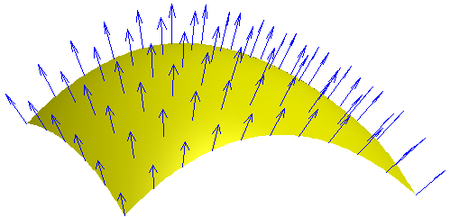
\includegraphics[width=0.65\linewidth]{normalfield.png}
            \caption*{}
\end {figure}
\end{frame}



\begin{frame}{Áttanlegir fletir} 

\begin {block}{Skilgreining \rtask{}}

Flöturinn $\cal S$ er sagður {\em áttanlegur} ef til er einingarþvervigrasvið
$\Nv$ á $\cal S$.  

\medskip
{\em Áttun} á áttanlegum fleti felst í því að velja annað af tveimur
mögulegum einingaþvervigrasviðum. 

\end{block}
\begin {figure}[h!]
 \centering
            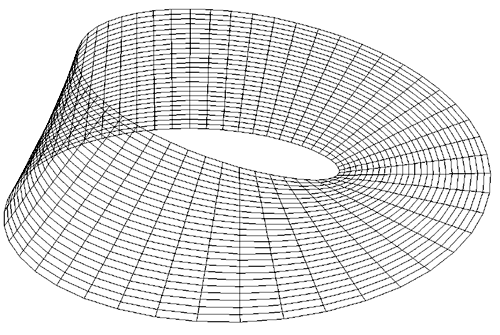
\includegraphics[width=0.40\linewidth]{mobius.png}
            \caption*{Möbiusarborði er ekki áttanlegur.}
\end {figure}
\end{frame}

\begin {frame}{}
 \begin {block}{Umræða \rtask{}}
  Ef áttanlegur flötur $\cal S$ hefur jaðar þá skilgreinir áttunin stefnu á jaðri $\cal S$. Venjan er að velja stefnu jaðarsins þannig að þegar gengið er eftir honum sé einingarþvervigrasviðið á vinstri hönd (hægri handar regla).
  
  \bigskip
  Ef tveir áttanlegir fletir hafa jaðar má splæsa þeim saman í áttanlegan flöt með því að líma þá saman á (hluta af) jöðrunum og gæta þess að jaðrarnir hafi andstæða stefnu á samskeytunum.
 \end {block}

\begin {figure}[h!]
 \centering
            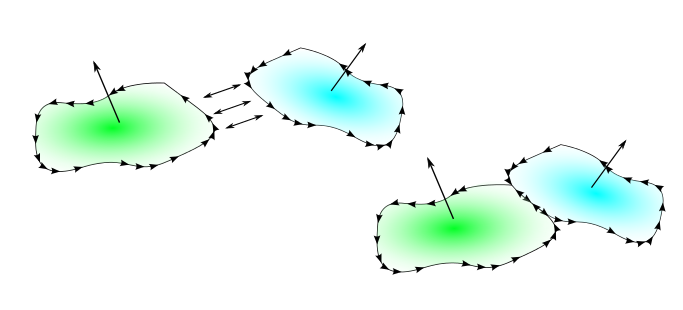
\includegraphics[width=0.95\linewidth]{joinsurf.png}
            \caption*{}
\end {figure}
\end {frame}

\begin{frame}{} 

\begin {block}{Setning \rtask{attun}}
 Gerum ráð fyrir að $\cal S$ sé áttanlegur
flötur og $\rv:D\subseteq\R^2\rightarrow \R^3$ sé regluleg stikun á
$\cal S$ (það er, $\frac{\partial \rv}{\partial u}$ og
$\frac{\partial \rv}{\partial v}$ eru samfelld föll af $u$ og $v$ og 
vigrarnir $\frac{\partial \rv}{\partial u}$ og
$\frac{\partial \rv}{\partial v}$ eru línulega óháðir).
Þá er 
$$\Nv=
\frac{\frac{\partial \rv}{\partial u}\times\frac{\partial
    \rv}{\partial v}}
{|\frac{\partial \rv}{\partial u}\times\frac{\partial
    \rv}{\partial v}|}$$
einingarþvervigrasvið á $\cal S$.  

\end{block}

\end{frame}



\begin{frame}{Heildi vigursviðs yfir flöt - Flæði} 

\begin {block}{Skilgreining og ritháttur \rtask{}}
 Látum $\cal S$ vera áttanlegan flöt stikaðan
af reglulegum stikaferli  $\rv:D\subseteq\R^2\rightarrow \R^3$ með
samfelldar hlutafleiður.  Látum $\Nv$ tákna einingarþver\-vigrasviðið
sem gefið er í \kaflanr.\ref{attun}.  Heildi vigursviðs $\Fv$ yfir flötinn $\cal S$ er
skilgreint sem 
$$\tvint_{\cal S} \Fv\cdot\Nv\,dS
=\tvint_D \Fv(\rv(u,v))\cdot \bigg(
\frac{\partial \rv}{\partial u}\times\frac{\partial \rv}{\partial
  v}\bigg)\,
du\,dv.$$
Slík heildi eru oft nefnd \emph{flæði vigursviðsins $\Fv$ gegnum flötinn $\cal S$.}

\bigskip
 Ritum $d\Sv=\Nv\,dS$.  Þá  er 
$$\tvint_{\cal S} \Fv\cdot\Nv\,dS=\tvint_{\cal S} \Fv\cdot\,d\Sv.$$
\end{block}

\end{frame}




\begin{frame}{} 

\begin {block}{Samantekt \rtask{}}
  
\begin{enumerate}
\item Ef $\rv:D\subseteq\R^2\rightarrow \R^3$ er stikun á $\cal S$ þá
  er $$d\Sv=\pm \bigg(\frac{\partial \rv}{\partial u}\times\frac{\partial
  \rv}{\partial v}\bigg)\,du\,dv.$$
\item Ef $\cal S$ er graf $z=f(x,y)$ þá er 
$$d\Sv=\pm\bigg(-\frac{\partial f}{\partial x},-\frac{\partial
  f}{\partial y},1\bigg)\,dx\,dy.$$
\item Gerum ráð fyrir að flöturinn $\cal S$ í $\R^3$ hafi þann eiginleika að
  ofanvarp hans á $xy$-planið sé eintækt eða með öðrum orðum hægt er
  að lýsa fletinum sem grafi $z=f(x,y)$.
Ef fletinum $\cal S$ er lýst sem 
hæðarfleti $G(x,y,z)=C$ þá er  
$$d\Sv=\pm\frac{\nabla G(x,y,z)}{|\nabla G(x,y,z)|}\,dS=
\pm\frac{\nabla G(x,y,z)}{G_3(x,y,z)}\,dx\,dy.$$
\end{enumerate}
Val á áttun felst í því að velja $+$ eða $-$ í formúlunum hér að
ofan.  

\end{block}

\end{frame}



\begin{frame}{} 

\begin {block}{Túlkun \rtask{}}
 Hugsum okkur að vigursviðið $\Fv$ lýsi streymi
vökva.  Hugsum svo flötinn $\cal S$ sem himnu sem vökvinn getur
streymt í gegnum.  Áttun á $\cal S$ gefur okkur leið til að tala um
hliðar flatarins og að vökvinn streymi í gegnum flötinn frá
einni hlið til annarrar.  Streymi vökvans gegnum flötinn (rúmmál per
tímaeiningu) er gefið með heildinu $\tvint_{\cal S} \Fv\cdot\Nv\,dS$
  þar sem streymi í stefnu $\Nv$ reiknast jákvætt.
\end{block}
\begin {figure}[h!]
 \centering
            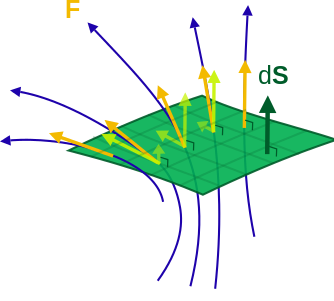
\includegraphics[width=0.45\linewidth]{flux.png}
            \caption*{}
\end {figure}
\end{frame}


\end{document}